% !TEX encoding = UTF-8 Unicode

\documentclass[a4j,12pt]{jsarticle}
\usepackage[dvipdfmx]{graphicx}
\usepackage{newtxtext} % アルファベットなどをTimesNewRomanで
%\usepackage{newpxtext} % アルファベットなどをPalatinoで
% 両方共コメントアウトするとComputer Modernで

\usepackage{listings}
\usepackage{okumacro}
\usepackage{graphicx}
\usepackage{url}
\usepackage{tabularx}
\usepackage{colortbl}
%\usepackage{float}
\usepackage{makeidx}
\usepackage{fouriernc}
\usepackage[deluxe]{otf}
\usepackage{mediabb}
\usepackage{amsmath}
\usepackage{moreverb}
%\usepackage{verbatim}

\usepackage{verbatim}
\usepackage{multirow}

% \usepackage[margin=2cm]{geometry}
\usepackage[top=20truemm,bottom=20truemm,left=30truemm,right=20truemm]{geometry}

\usepackage{dcolumn}
\usepackage{ascmac}
\usepackage{color}
\usepackage{eclbkbox}
\usepackage{itembkbx}
\usepackage{enumerate} %箇条書きを装飾する際に使う
\usepackage{multicol}
% 自分で追加
\usepackage{comment}%複数行コメントアウト
\usepackage{multirow}%表結合
\usepackage{here} %図や表などを強制的に出力
\usepackage{fancybox} %四角で囲む
\usepackage{boxedminipage} %箇条書きを四角で囲む
\usepackage{caption} %キャプションの設定
\usepackage{longtable} %表がページをまたがるときの処理
\usepackage{slashbox} %表に斜線を入れる
% \usepackage{emathT} %表に斜線を入れる
\usepackage{framed} %箇条書きを枠で囲む
\newcolumntype{I}{!{\vrule width 1.5pt}}% 縦線の一部を太くする(Iで指定する)
% 横線の一部を太くする(wlineで範囲を指定する)
\newlength\savedwidth
\newcommand{\wcline}[1]{\noalign{\global\savedwidth\arrayrulewidth\global\arrayrulewidth 1.5pt} \cline{#1}
\noalign{\global\arrayrulewidth\savedwidth}}
\usepackage{lscape} % 表を横向きに表示

% 数字を丸で囲む
\def\MARU#1{\leavevmode \setbox0\hbox{$\bigcirc$}%
\copy0\kern-\wd0 \hbox to\wd0{\hfil{#1}\hfil}}
%%%%%%%%%%%%%%%%%%%%%%%%%%%%%%%%%%


\makeatletter % プリアンブルで定義開始
\renewcommand{\presectionname}{第}
\renewcommand{\postsectionname}{章}
\renewcommand{\appendixname}{付録}


%章,節,項の文字サイズ
\def\section{\@startsection {section}{1}{\z@}{3.5ex plus -1ex minus -.2ex}{2.3 ex plus .2ex}{\Large\bf}}
\def\subsection{\@startsection {subsection}{1}{\z@}{3.5ex plus -1ex minus -.2ex}{2.3 ex plus .2ex}{\Large\bf}}
\def\subsubsection{\@startsection {subsubsection}{1}{\z@}{3.5ex plus -1ex minus -.2ex}{2.3 ex plus .2ex}{\large\bf}}


\usepackage{caption} %キャプション文字サイズ(大)
\captionsetup[figure]{font=normalsize}
\captionsetup[table]{font=normalsize}
\captionsetup[equation]{font=normalsize}

% 図の番号を"<章.節の番号> - <図の番号>" へ
\renewcommand{\thefigure}{\thesubsection-\arabic{figure}}
% 表の番号を"<章.節の番号> - <表の番号>" へ
\renewcommand{\thetable}{\thesubsection-\arabic{table}}
% 数式の番号を"<章.節の番号> - <数式の番号>" へ
\renewcommand{\theequation}{\thesubsection-\arabic{equation}}

% 章と節が進むごとに図の番号をリセットする
\@addtoreset{figure}{subsection}
% 章と節が進むごとに表の番号をリセットする
\@addtoreset{table}{subsection}
% 章と節が進むごとに数式の番号をリセットする
\@addtoreset{equation}{subsection}

% 章と節が進むごとに注釈の番号をリセットする
% \@addtoreset{footnote}{subsection}

% 注釈の設定
\renewcommand{\thefootnote}{\fnsymbol{footnote}}


\makeatother % プリアンブルで定義終了


%%%%%%% グラフックパス
\graphicspath{{fig/}}
 
\makeindex
\begin{document}

% フォントサイズ・行間
\fontsize{20pt}{15pt}\selectfont

% 表紙
\thispagestyle{empty} % ページ番号削除

\begin{center}
\huge
\vspace*{\stretch{2}}

2019年度 卒業論文\\[50pt]
\HUGE

コーヒー抽出に関する音声認識可能な\
Webレシピの開発\\
\huge
\vspace*{\stretch{6}}
指導教員 須田 宇宙 准教授\\[40pt]
千葉工業大学 情報ネットワーク学科\\[10pt]
須田研究室\\[60pt]
1632130 \hspace{50pt} 氏名 肥田雄也\\[75pt]
\end{center}

\begin{flushright} 
\huge
提出日 2020年1月25日
\vspace{\stretch{2}}
\end{flushright}

\newpage
\thispagestyle{empty} % ページ番号削除
%\input{input0}

% フォントサイズ・行間
\fontsize{11pt}{15pt}\selectfont

% 目次
\pagenumbering{roman}
\setcounter{page}{1} % ページ番号1
\setcounter{tocdepth}{3}

\newpage
\tableofcontents
%\pagestyle{empty}

%\thispagestyle{empty} 

\newpage
%\thispagestyle{empty}
\listoffigures

\newpage
%\thispagestyle{empty}
\listoftables






%%%%%%%%%%%%%%%%%%%%%%%%%%%%%%%%%%%%%%%%%%%%%%%%%%
%ここから本文
\newpage
\pagenumbering{arabic}
\section{緒言}
\setcounter{page}{1} % ページ番号1
「悪魔のように黒く、地獄のように熱く、天使のように純粋で、愛のように甘美である。」これはフランスの外交官である,シャルル=モーリス・ド・タレーラン=ペリゴールが遺したコーヒーの名言である.
コーヒーはただの飲料物でありながらも,長い年月をかけて愛され,世界の人々を魅了してきた.
%音楽は国境を超えると言われている.音は人間の感覚に直接刺激を与え,その形は国を超えて愛されるものである.その結果,日々世界中でコンサートやライブが開催され,多くの客を動員している.

それは日本も例外ではない.
江戸時代初期に長崎の出島に持ち込まれた際は,一部の人間しか飲用はできなかったが,明治時代に文明開化が起きるとみるみるうちに一般層に普及していった.
現代では,国際機関コーヒー機関(ICO)の「世界の国別コーヒー消費量」で4位を記録しているほどである.
%また,音楽は体を動かす必要がないため,老若男女多くに好かれるものであるといえる.音楽を生業にする人のみならず,趣味として音楽に関与することを上げる人も多くその人気は高い.さらに,誰もが幼少期から歌や楽器演奏等,様々な形で音楽と関わっており,音楽は多くの人にとって身近なものであることが伺える.
%楽器を演奏する人も多くいるがその中でもピアノが人気であるといえる.ピアノは歌や他の楽器との相性がいいことから誰もが一度は関わったことがあるだろう.
%私はこの度の研究に際して,ピアノをテーマにした研究に興味を持った.
%日本ではピアノの奏者が約200万人いると言われており,それに従い個人から大手まで多くのピアノ教室が存在している.

また近年,高品質なコーヒーをより良い淹れ方で味わうサードウェーブコーヒーが流行している.

%問題点
しかし,美味しいコーヒーを淹れるためには抽出器具に合わせたテクニックが必要である.
抽出手順や,器具ごとの特徴の違いなどから学習の難易度が高くなり,コーヒーを淹れることの敷居も高くなっている.
また,実際の抽出中は,両手が塞がっていたり手が濡れているなど,レシピブックを捲ることに対する障害も多い.
クックパッドやmacaroniのような,音声認識でレシピを閲覧できるWebサイトは複数存在するが,コーヒーの抽出に特化したサイトは無いことも問題点である.

%目的
そこで,様々な抽出器具のレシピが閲覧可能であり,音声認識によってページ移行が可能なWebレシピがあれば,問題点の改善に繋がると考えた.
本研究では上記のWebレシピを作成することを目的とする.

%%%%%%%%%%%%%%%%%%%%%%%%%%%%%%%%%%%%%%%%%%%%%%%%%%

\newpage
\section{\large{コーヒーについて}}
本章では,コーヒーの歴史や流行について説明する.
\subsection{\large{コーヒーとは}}
コーヒーとは,コーヒーノキという樹木から採取される種子を焙煎し,お湯等で成分を抽出した飲料物である.主に北回帰線と南回帰線を挟むコーヒーベルトと呼ばれる地域で栽培されており,数百種類の品種が存在する.商業生産としては,高品質であるが栽培の難しいアラビカ種がおよそ60%前後を占めている.アラビカ種は,スペシャルティコーヒーと呼ばれる高品質コーヒーの主要製品であり,多くのカフェで提供されている.残りの40%はロブスタ種が占めており,こちらは品質はアラビカ種に劣るが耐病性に優れ,大量生産向きであり缶コーヒーやインスタントコーヒー等に用いられる.

%抽出方法についても日本の純喫茶でよく見られるプアオーバーや,サイフォンの他に,フレンチプレス,エスプレッソ,ソロフィルターなど,その目的や表現したい風味に従い,多くの数が存在し使い分けられている.
%ピアノとは,弦をハンマーで叩くことで発音する弦楽器の一種である.88個の鍵があり,鍵を押すことで対応する弦をハンマーが叩き,音が発生する仕組みである.打楽器と弦楽器の特性を持ち合わせていることから打弦楽器に分類される.その音域は非常に広く,オーケストラの全音域よりも広い.汎用性が高く,演奏目的のみならず音楽教育や作曲等,様々な目的で利用される.そのためピアニストのみならず,他の楽器の演奏者や声楽家,作曲家,指揮者,教育指導者等様々な場面でピアノ演奏技術が必要とされる.
%ピアノにはいくつかの種類があり,グランドピアノ・アップライトピアノ・エレクトリックピアノ・電子ピアノなどそれぞれの目的に応じて使い分けることが可能である.
\subsection{\large{コーヒー(アラビカ種)の起源と伝搬の歴史}}
コーヒー(アラビカ種)はエチオピアのアビシニア高原にて発見された.その後,アラビアに伝播しオランダの貿易商人達の手によってアフリカやアジアへと広がっていき,商業用生産が活発になる.
アフリカやアジア各国にコーヒーが広がり,フランスに至ると,とある海軍兵士がコーヒーの苗木を当時フランス領であったマルティニーク島に持ち出すことになる.
こうしてラテンアメリカにもコーヒーは広がり,温暖でコーヒーの栽培に特に適した北回帰線と南回帰線を挟むコーヒーベルトにおいて栽培は進んでいった.
現代でも,コーヒーベルト各国はコーヒーシェアのほとんどを占めている.
グアテマラ・ブラジル・コロンビア・スマトラなどは,コーヒーを普段飲まない人でも聞き馴染みのある生産地であろう.

%ピアノはイタリアのクリストフォリ(1655\UTF{FF5E}1731)が作成した.ピアノが存在する前はチェンバロという,ピアノに似た楽器が存在していた.チェンバロは1500年に作られた楽器で弦を爪ではじいて音を出すものであった.
%しかし,チェンバロは音の強弱がわかりづらく,表現力に乏しいという問題点があった.
%それを不満に思ったのがクリストフォリである.クリストフォリは1700年ごろに図\ref{fig:pianosikumu}のようにハンマーで打って鳴らすという現在のピアノの原型を作りあげた.彼はこのメカニズムを備えた楽器をグラヴィチェン・コル・ピアノ・エ・フォルテ(弱音も強い音も出せるチェンバロ)と名付けた.それが普及し,現在もピアノは世界中で使用されているのである.

\subsection{\large{コーヒー(ロブスタ種)の起源と伝搬の歴史}}




\begin{figure}[htbp]
 \begin{center}
  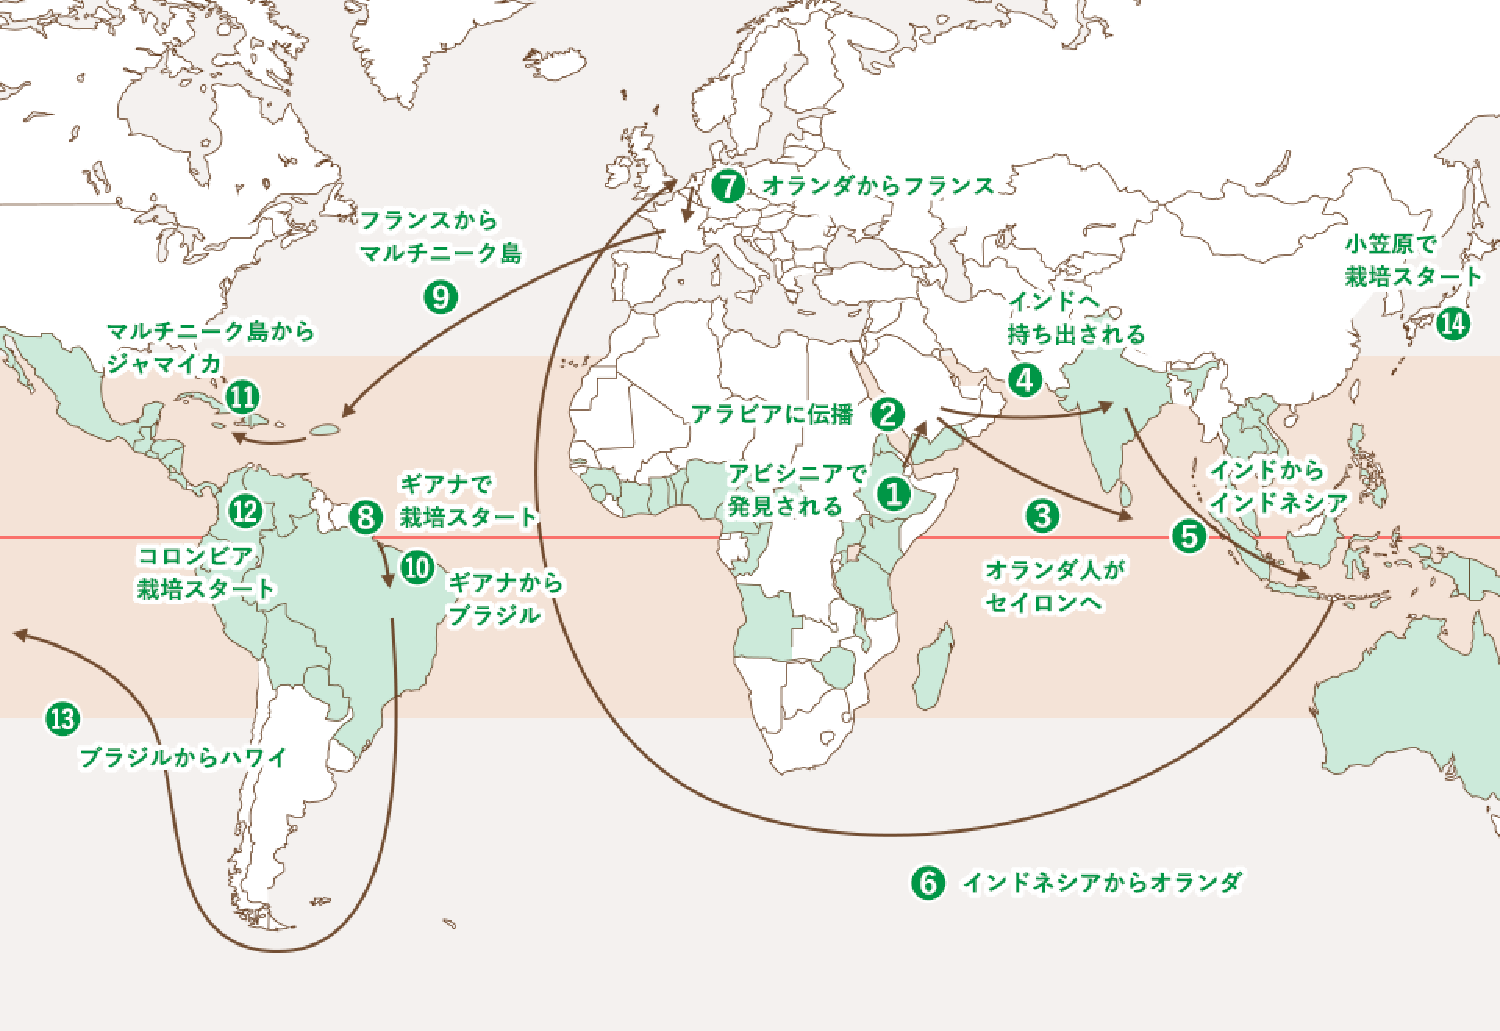
\includegraphics[width=80mm]{figure/map.pdf}
 \end{center}
  \caption{UCCホームページより:コーヒーの軌跡}
  \label{fig:pianosikumu}
\end{figure}


\newpage
\subsection{\large{コーヒーの流行について}}
ここでは,コーヒーの流行を時代別に説明する際に使われる,ウェーブという表現について説明する.
コーヒーはその時代ごとに求められる姿を変え,ファーストウェーブ(第一の波),セカンドウェーブ(第二の波),サードウェーブ(第三の波)へとシフトしていく.
このウェーブという表現は,明確な時間の括りを示すものではないが,流行りの移り変わりとしてコーヒーを語る上で多く用いられる.
\subsubsection{\large{ファーストウェーブ}}
ファーストウェーブ(第一の波)の到来と期間は,19世紀後半\UTF{FF5E}1960年頃と言われている.
この流行はコーヒーの大量消費時代であり,真空保存パックの発明や,インスタントコーヒーの発売などが起きた時代でもある.
真空保存パックの発明は,コーヒーの保存期間を劇的に延長し,地方だけでなく大都市でも新鮮なコーヒーが飲めるようになった.
インスタントコーヒーの発明は,コーヒーを楽しむことをより手軽な事とした,第一次・第二次世界大戦においても多くの兵士が愛飲したと言われている.
しかしその反面,この時代のコーヒーは風味がとても乏しく,粗悪品が多く出回る時代でもあった.
\subsubsection{\large{セカンドウェーブ}}
セカンドウェーブ(第二の波)の到来と期間は,1960年頃〜2000年頃と言われている.
ファーストウェーブの際に,一般的かつ手軽な飲み物として普及が進んだコーヒーであったが,普及が進むとともに劣悪な品質が問題化した.
そして,シアトル系コーヒーチェーンを代表とする,より味にフォーカスした流行が起こる,それがセカンドウェーブである.
コーヒーそのものだけでなく,カフェラテなどのエスプレッソドリンクもシアトル系カフェの台頭とともに普及し,現代におけるコーヒー事情の基盤を作ったと言っても過言ではない流行である.
\subsubsection{\large{サードウェーブ}}
サードウェーブ(第三の波)の到来と期間は,2000年頃〜現在も続くと言われている.
セカンドウェーブの際に,品質についての意識が向上したことを皮切りに,高品質かつそのコーヒーの生まれや,農園,淹れ方,加工法など全てにおいて重視される流行が訪れる事となる.それがサードウェーブコーヒーである.
コーヒーの抽出技術を競う大会や,カップオブエクセレンスと呼ばれるその年のコーヒーで最高品質の物を決める評議会が開催されるなど,より一杯の価値にフォーカスされている流行である.
また,昔から日本のカフェで行われてきたハンドドリップは,日本でこそ当たり前の光景だったものの,海外では目新しいものであり,この流行とともに注目を集めていく事となる.
%%%%%%%%%%%%%%%%%%%%%%%%%%%%%%%%%%%%%%%%%%%%%%%%%%

\newpage
\section{\large{抽出方法と抽出器具について}}
本章では,基本的な抽出方法や抽出器具を説明する.

\subsection{\large{抽出方式}}
ここでは,抽出の仕組みとも言える抽出方式を説明する.
\subsubsection{\large{浸漬式}}
浸漬式は,コーヒープレスやコールドブリューに代表される抽出方式である.
名前の示す通り,コーヒー豆をお湯に浸し,適切な時間漬けておくことで,風味を引き出す.
コーヒーは抽出を過剰に行った場合,雑味やエグ味まで抽出されてしまうため,抽出にかかる時間を適切に管理することが,浸漬式では特に重要である.
比較的長時間の抽出になるため,粗挽きの豆を使用するのが一般的である.
\subsubsection{\large{透過式}}
透過式とは,プアオーバーやケメックスに代表される抽出方式である.
浸漬式とは異なり,抽出されたコーヒーはフィルターを介し,豆とお湯が分離されサーバーに落とされていく.
\subsubsection{\large{高圧抽出式}}


\subsubsection{\large{真空濾過式}}


\newpage
\subsection{\large{抽出器具}}
ここでは,数多く存在すつ抽出器具の一例を説明する.
\subsubsection{\large{コーヒープレス}}
コーヒープレスは,フレンチプレスと呼ばれる器具に,挽いたコーヒー豆とお湯を入れ,時間をかけて抽出を行う器具である.
紅茶でいうティープレスのように,抽出時間経過後は上からステンレスフィルターを押し下げ,豆と液体を分離することによって,抽出を完了させる.
仕上がりは.多少の粉末感を残すものの,濃厚でまろやかな味わいである.
ステンレスフィルターを使用するため,コーヒーのオイルが吸収されず,コーヒー豆本来の味が楽しめることも利点の一つである.
\subsubsection{\large{プアオーバー}}
プアオーバーは,別名ハンドドリップとも呼ばれており,日本の喫茶店で多く提供されてきたことから,日本人に特に馴染みの深い抽出器具と言える.
フィルターの上に挽いた豆を置き,お湯を回しかける事によって,下部のグラスサーバーにコーヒーを抽出していく.
フィルターを介しているため,出来上がりは,粉末感は殆どなくクリーンな味わいになりやすい.
また,お湯の注ぐタイミングや蒸らしの時間の掛け方などにより,様々な流派が存在し,淹れた人によって大きく風味が変化する事も特徴の一つである.
\subsubsection{\large{コーヒープレス}}
コーヒープレスは,フレンチプレスと呼ばれる器具に,挽いたコーヒー豆とお湯を入れ,時間をかけて抽出を行う器具である.
紅茶でいうティープレスのように,抽出時間経過後は上からステンレスフィルターを押し下げ,豆と液体を分離することによって,抽出を完了させる.
仕上がりは.多少の粉末感を残すものの,濃厚でまろやかな味わいである.
ステンレスフィルターを使用するため,コーヒーのオイルが吸収されず,コーヒー豆本来の味が楽しめることも利点の一つである.
\subsubsection{\large{エスプレッソ}}
エスプレッソは,イタリアを発祥とする飲み方であり,水蒸気やピストンなどで圧力をかけ,短い時間で抽出されたコーヒーのことを指す.
自動式・半自動式・ピストン式など様々なエスプレッソマシンが存在するが,使用者自身でフィルターに豆を押し込み,機械によって気圧をかける半自動式が最も一般的である.
仕上がりは極めて濃厚であり,そのままの状態で飲む以外にも,ミルクを追加しカフェラテ・カプチーノとして提供されることが多い.
\subsubsection{\large{ソロフィルター}}
ソロフィルターは,カフェ等ではあまり提供されないが,コーヒーを初めて淹れる人でも簡単に抽出でき,入門用に最適な器具の一つである.
ステンレスフィルターの上に挽いたコーヒー豆を置いた後,複数の極細の穴があるパーツに規定量のお湯を注ぐだけで,適切な湯量が豆に注がれ続ける.
容量は1杯分のコーヒー豆しか入らないため,大人数分のコーヒーを抽出するには不向きだが,粉末感の殆どない高品質なコーヒーを手軽に味わえるため,
コーヒーを学び始めの人や,朝の忙しい時間でも簡単に抽出することができる.
\subsubsection{\large{サイフォン}}
サイフォンは,科学の実験器具のような形状をした抽出器具であり,数ある抽出器具の中でも特に見栄えの良い器具として,注目を集めている.
お湯を熱したことによる蒸気圧を使用し,真空に近い状態を作り出すことで,コーヒーが器具の内部を上下し,フィルターを通して濾過される.日本の喫茶店でも多く取り入れられていたため,馴染みの深い抽出器具でもある.
従来は加熱にアルコールランプを使用していたが,最近では電気式が主流となっている.
\subsubsection{\large{クレバードリッパー}}
クレバードリッパーは,近年新たに提案された浸漬式と透過式を合わせた抽出器具である.
コーヒープレスと同様に,コーヒー豆をお湯に浸し適切な時間をおいた後,ペーパーフィルターを通し,豆とお湯を分離する抽出方法をとる.
味わいは,浸漬式のマイルドさと,透過式のスッキリさを併せ持っている.一度に多くのコーヒーを抽出できるほか,プアオーバーのような複雑な工程を踏まないため,比較的簡単に抽出を行うことができる.
\subsubsection{\large{エアロプレス}}
エアロプレスは,その名の通り空気圧を使用した抽出器具である.開発されたのは2005年であり,数多くの抽出器具の中でも特に直近に提案された器具である.
注射器のような形状をしており,利用者自身が器具を押し込むことによって,空気圧を調整し抽出を行う.
抽出時間が短いこと,味わいが濃厚であることが特徴である.
2005年という直近の開発でありながら,様々なカフェで提供されている他,エアロプレスに特化した,抽出技術を競う大会が開催されたりと,シェアを順調に伸ばしている.
%%%%%%%%%%%%%%%%%%%%%%%%%%%%%%%%%%%%%%%%%%%%%%%%%%

\newpage
\section{\large{コーヒー抽出の学習方法}}
本章では,ピアノの基本的な指導方法を説明する.

\subsection{\large{抽出の基本的な学習方法}}
ピアノには特定の指導法はなく,指導者の方針や教k室ごとにその方針は異なる.そのため,ピアノの上達は先生の指導方法によって大きく変化する.

熟練度は低くても指導が得手である指導者もいれば,熟練度が高くても指導が不得手な指導者もいる.
各指導者の性格,腕前,環境など様々な要因があり,多種多様であるといえる.

\subsection{\large{コーヒーの学習が可能なWebサイトついて}}
前述したようにピアノには決まった指導法がなく個人のピアノ教室となると,教室ごとの特性が顕著にみられるようになる.

しかし,指導者と生徒が1対1であることが多いため,その生徒に合わせた指導ができることは共通している.
教室によっては,生徒に合わせた曲を選択したり,学習する順番を考慮したりする場合もある.

\subsection{\large{既存の音声認識可能なWebレシピについて}}
前述したようにピアノには決まった指導法がなく個人のピアノ教室となると,教室ごとの特性が顕著にみられるようになる.

しかし,指導者と生徒が1対1であることが多いため,その生徒に合わせた指導ができることは共通している.
教室によっては,生徒に合わせた曲を選択したり,学習する順番を考慮したりする場合もある.

%%%%%%%%%%%%%%%%%%%%%%%%%%%%%%%%%%%%%%%%%%%%%%%%%%


%%%%%%%%%%%%%%%%%%%%%%%%%%%%%%%%%%%%%%%%%%%%%%%%%%

\newpage
\section{\large{プログラミング言語と音声認識ついて}}
本章では,システムを制作する上で利用するプログラミング言語について説明する.
\subsection{\large{HTML・CSSとは}}
Pythonとは,プログラミング言語の1つである.コードがシンプルで,初心者でも扱いやすいことが特徴である.文法が単純なため,プログラムの可読性が高いことがあげられる.
多くのハードウェアとOSに対応しており,オブジェクト指向・命令型・手続き型・関数型などの形式でプログラムを書くことができる.
この特性から,PythonはWebアプリケーション開発やデスクトップアプリケーションなどの開発をはじめ,自動処理や統計・解析など幅広く使われるようになった.
プログラミング作業が容易で効率的であることから,ソフトウェア開発企業にとって時間短縮や人数削減が見込めるとして多く利用されている.
近年,機械学習が多く用いられるようになり,Pythonが利用される場面がより多くなっている.

\subsection{\large{音声認識とは}}
\subsubsection{\large{音声認識の仕組み}}
\subsubsection{\large{WebSpeechAPI}}

\subsubsection{\large{音声認識を可能にするJavaScriptについて}}
本システムでは,楽譜を解析し,そのデータをもとに音階を割り出し,表示するシステムを開発している.画像開発を行っている上で利用しているのはOpenCVであるが,OpenCVは日本語表示ができないという特徴がある.そのため,プログラム上では英語表記の音階を扱わなくてはいけないが,出力する際には一般的に用いられるイタリア語表記の音階を表示しなくてはいけない.

そこで本研究ではPythonの画像処理ライブラリであるPillow(PIL)を用いて日本語の出力を行った.Pillowとは,PIL(Python Image Library)からフォークされた画像処理ライブラリである.OpenCVのような高度な画像処理はできないが,リサイズや回転,トリミングなどの単純な画像加工は行うことができる.実際にPillowを用いて加工を行った画像を図\ref{fig:pillow}で示す.基本的には画像の読み込み,処理,保存に使われる他,図形の描画などを行う.日本語に対応しているため,本研究ではPillowを利用して音階の表示と画像の保存を行う.


\subsubsection{\large{音声認識によるページ移動}}
そして,音階を求める上で重要なのは五線の中央の線である.五線の中央は各音階を求める上で基準となる.五線の中央を図\ref{fig:gosentyuuou}に示す.
五線の中央は分割した五線を格納した配列の3番目の値を取り出すことで求めることができる.
各五線の中央の線から,音符の楕円の中央までの距離を計算し,各音階の中で最も近い値の音階を出力する.

%%%%%%%%%%%%%%%%%%%%%%%%%%%%%%%%%%%%%%%%%%%%%%%%%%

\newpage
\section{\large{本研究で開発するWebレシピの概要}}
本章では,実際に制作するシステムについて説明する.
\subsection{\large{コンセプトについて}}
\subsection{\large{実装機能}}
本研究で実装する機能は音階の自動表示である.楽譜をスキャンし,その画像をOpenCVで解析することで楽譜の五線と音符の位置を割り出す.その座標から音階を割り出し,楽譜に表示させることを最終目的とする.本システムのフローチャートを図\ref{fig:furo-}に示す.

\begin{figure}[htbp]
 \begin{center}
  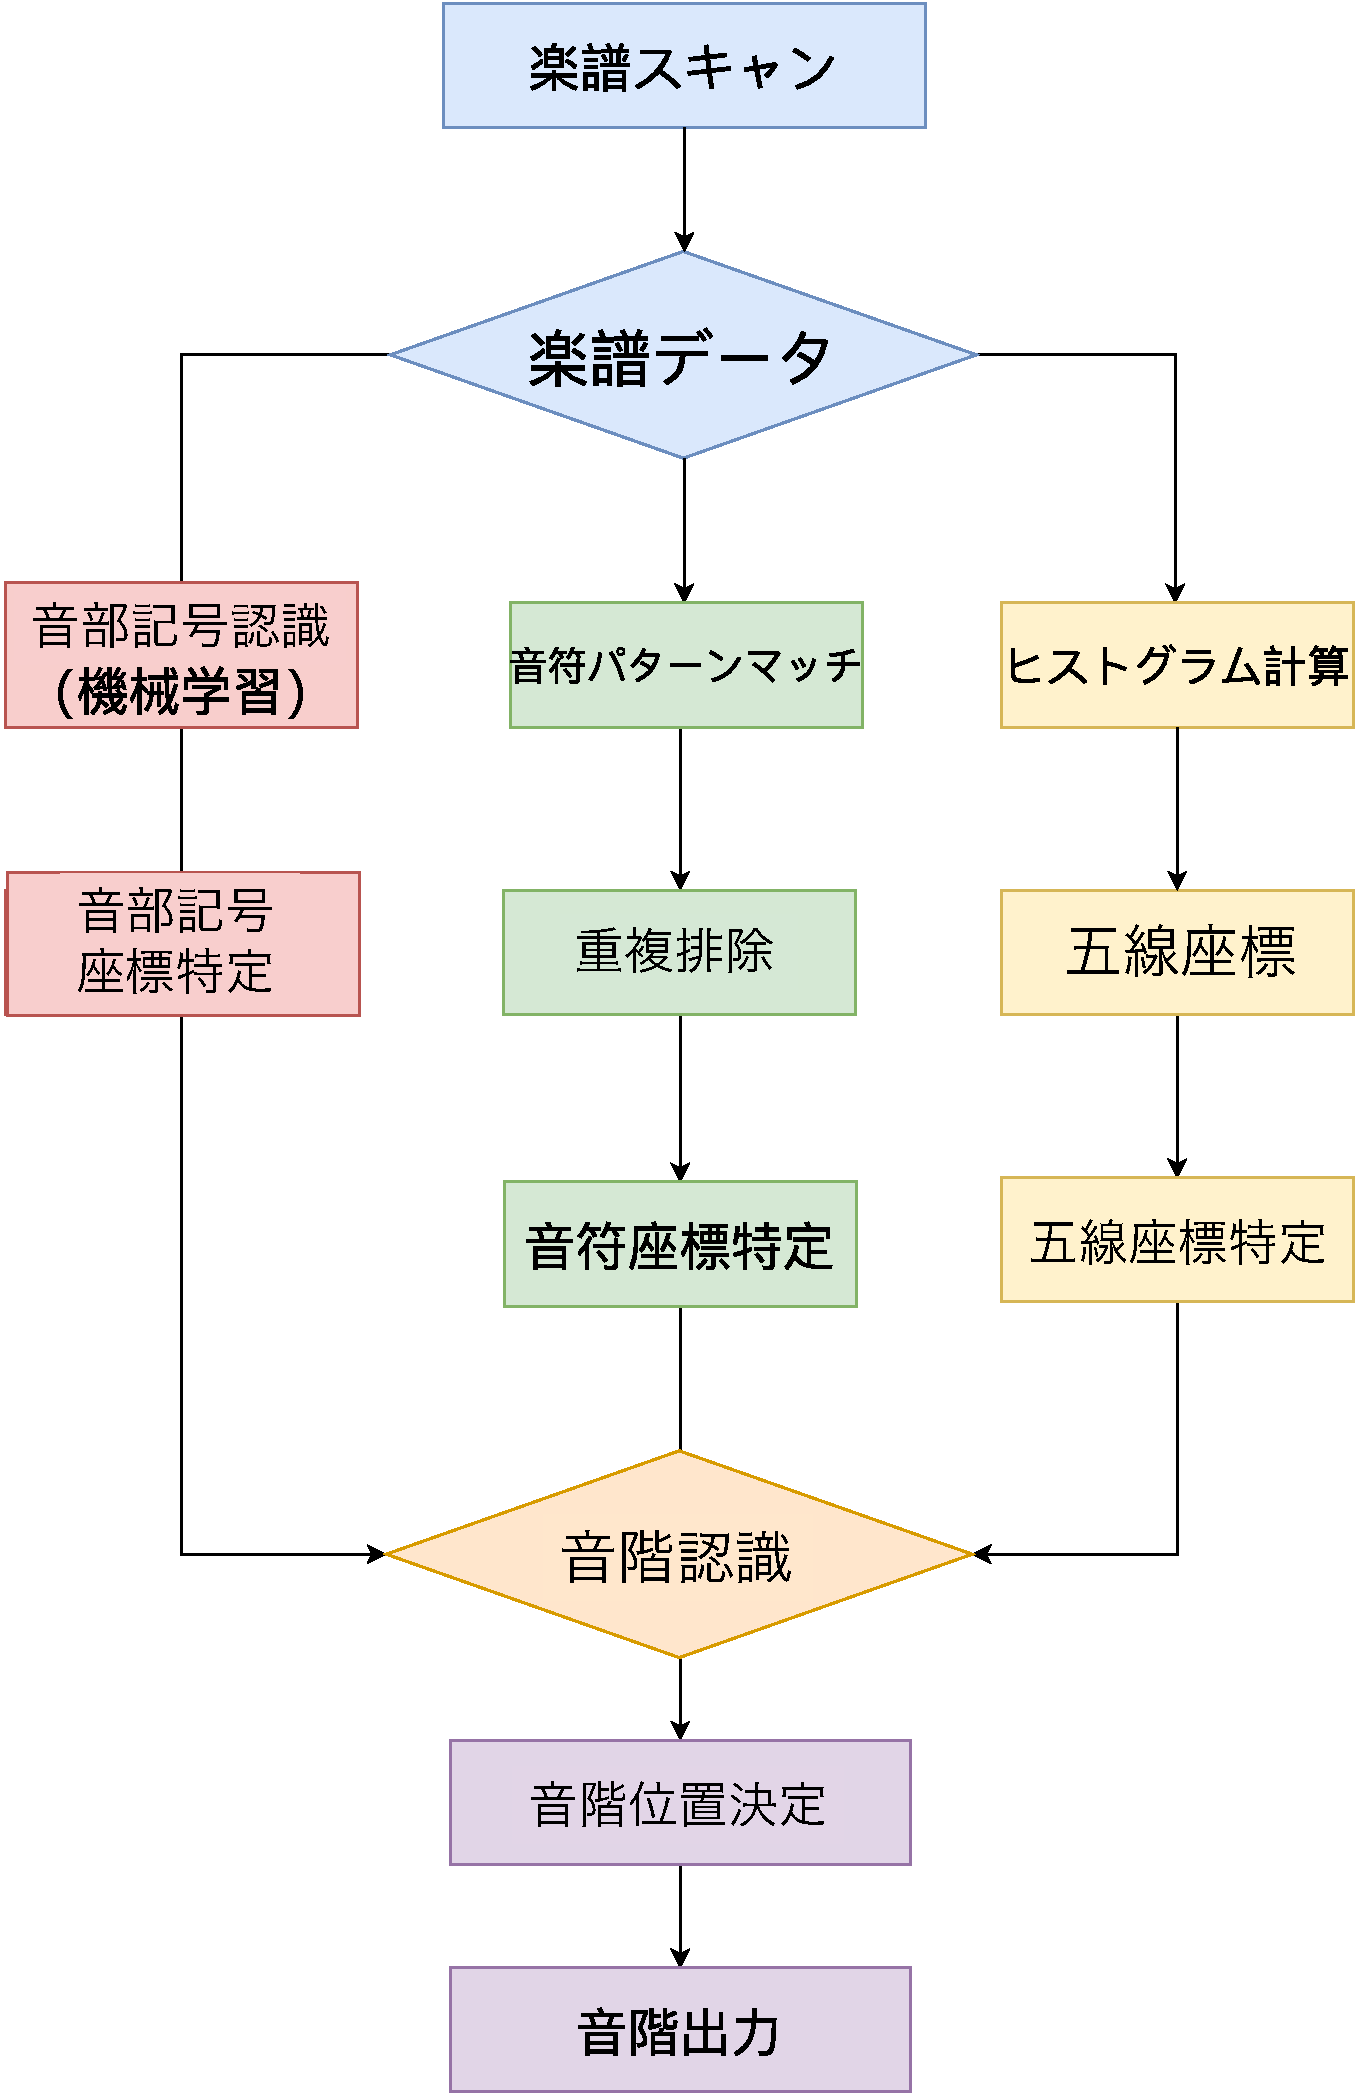
\includegraphics[width=90mm]{figure/furo-.pdf}
 \end{center}
 \caption{本システムのフローチャート}
 \label{fig:furo-}
\end{figure}


\newpage
\subsection{\large{本Webレシピのページ構成について}}
楽譜は音部記号と五線と音符で構成されている.つまり,その3要素を抽出できれば音階を割り出すことができるということになる.
音部記号は機械学習を用いる.機械学習はポジティブ画像(学習対象が存在している画像)とネガティブ画像(学習対象が存在してない画像)から特徴点を抽出し,対象の画像から学習対象があるか判別するものである.TrainingAssistantというカスケード分類器を利用することでポジティブ画像,ネガティブ画像,どちらにも属さない画像(関係ない記号である等)に分類することができる.本研究では,そのデータを利用することで機械学習を行う.
ト音記号の特徴を学習させることで,ト音記号のみの楽譜にも,ヘ音記号が混じった楽譜にも対処することができる.

五線は各ピクセルを解析し,ヒストグラムを生成することで座標を割り出す.各X軸の黒点の数をカウントし,一定の個数以上の黒点が検出されたX軸には五線が存在している確率が極めて高いと推測される.それを利用して座標を記録する.

音符の検出にはパターンマッチを利用する.楕円の形を検出対象とし,音符の符頭を割り出す.閾値を低めに設定して検出し,多重マッチングをしている箇所を抽出することで,正確に符頭を割り出す.また,検出した楕円の中央座標を記録することで正確に音階を割り出せるようにする.


\subsubsection{\large{抽出器具選択画面}}
OpenCVとPythonを利用して実装していく.楽譜認識は音部記号,五線,音符の順に検出していき,その情報を利用して音階の出力を試みる.

\subsubsection{\large{レシピ閲覧画面}}
OpenCVとPythonを利用して実装していく.楽譜認識は音部記号,五線,音符の順に検出していき,その情報を利用して音階の出力を試みる.

\newpage.


%%%%%%%%%%%%%%%%%%%%%%%%%%%%%%%%%%%%%%%%%%%%%%%%%%



%%%%%%%%%%%%%%%%%%%%%%%%%%%%%%%%%%%%%%%%%%%%%%%%%%

\newpage
\section{\large{結言}}
音楽は趣味や仕事の面で多くの人が関わり,古代から現代まで長く続いている文化である.職種としてのみならず,趣味としても多くの人にあげられる音楽は世界共通の言語なのである.

特にピアノは歌やその他の楽器との相性が良いことから楽器としては最も多くの人に関与するものであり,その分奏者人口も多いことが挙げられる.
ピアノを学ぶ上で楽譜は必要不可欠な要素であり,今後も多くの人々が楽譜と関わることになる.しかし,ピアノの楽譜は初心者にとって難しく,挫折の要因の1つとして挙げられる.

そこで本研究では,ピアノ指導者が各音符に手書きで音階を書き込む際,指導者にとって時間的コストがかかっている現状を問題点とし,その対策として実際に音階表示補助システムを開発し,ピアノ指導者に評価してもらうことを目的とした.

実際にOpenCVとPythonを利用し,音階を認識するシステムを制作した.実際に音階を表示し,ピアノ指導者の評価を得た.本システムを導入するかの差があるとはいえ,時間的コスト削減の面で本システムは大きく貢献できることがわかった.

また,今後の展望としては音階の表示のみならず,音階表示のパターンを変化,音階表示以外の視覚サポート,音によるサポート等ができるとより良いシステムになる.


%%%%%%%%%%%%%%%%%%%%%%%%%%%%%%%%%%%%%%%%%%%%%%%%%%

\newpage
\section*{謝辞}
本研究の遂行及び本論文の作成にあたり,須田研究室の仲間に深く感謝の意を表します.そして,何よりも本論文の作成にあたり,多大なる御指導及び御助言を頂きました須田宇宙准教授に深く感謝の意を表します.

%%%%%%%%%%%%%%%%%%%%%%%%%%%%%%%%%%%%%%%%%%%%%%%%%%
%参考文献
\newpage
\section{\large{参考文献}}\label{参考文献}
\begin{thebibliography}{9}
%\bibitem{kawahara}名前, ``書籍名'', 出版, Vol71, No11, 年, pp197-203
\bibitem{Railshon1} 
総務省統計局 , ``平成23年社会生活基本調査'', \url{http://www.stat.go.jp/data/shakai/2011/}\\
\bibitem{Railshon2} 
早稲田大学理工学部情報学科  板東慶一郎, ``楽譜認識を活用した演奏支援ソフトウェア'', \url{file:///Users/masuda/Downloads/1g01p08220(5).pdf}\\
\bibitem{Railshon3} 
OpenCV team,``OpenCV'',\url{https://opencv.org/}\\
\bibitem{Railshon4} 
Python Software Foundation, ``Python'', \url{https://www.python.org/}\\
\bibitem{Railshon5} 
神奈川工科大学 情報学部 情報工学科 信号処理応用研究室 , ``標準画像/サンプルデータ'', \url{http://www.ess.ic.kanagawa-it.ac.jp/app_images_j.html#image_dl}\\

\bibitem{Railshon6} 
paulrosen , ``abcjsデモページ'', \url{https://abcjs.net/abcjs-editor.html}\\

\bibitem{Railshon7} 
KoheiShitaune,``TrainingAssistant'',\url{https://github.com/shkh/TrainingAssistant}\\

\bibitem{Railshon8} 
教育芸術社 市川都志春 編著,``こどものバイエル第1集'',2004年10月30日初版発行,2018年3月第34版発行,pp5\\

\bibitem{Railshon9} 
株式会社ドレミ楽譜出版社 橋本晃一 編著,``中級レベルで弾けるクラシック名曲ピアノ曲集'',1994年1月初版発行,2007年2月20日第7版発行,pp26-27\

\end{thebibliography}
%%%%%%%%%%%%%%%%%%%%%%%%%%%%%%%%%%%%%%%%%%%%%%%%%%
%付録
\newpage
\newgeometry{left=2cm,bottom=2cm}
\appendix
\section{作成したプログラム}

\section*{Square.py}
\label{Square.py}
\listinginput{1}{program/Square.py}
\newpage

\section*{Circle.py}
\label{Circle.py}
\listinginput{1}{program/Circle.py}
\newpage

\section*{Decision.rb}
\label{Decision.rb}
\listinginput{1}{program/Decision.rb}
\newpage

\section*{Line.py}
\label{Line.py}
\listinginput{1}{program/Line.py}
\newpage

\section*{index.py}
\label{index.py}
\listinginput{1}{program/index.py}
\restoregeometry

\end{document}